\begin{exercise}
\begin{figure}[H]
\centering
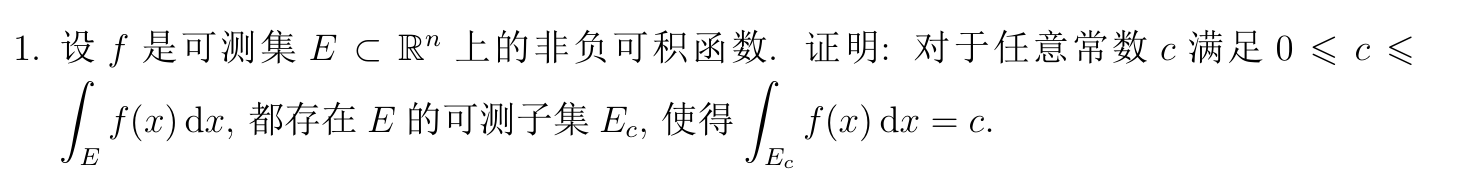
\includegraphics[width=\textwidth]{hw13-2025060311.png}
% \caption{}
\label{}
\end{figure}
\end{exercise}
$E_{y}\coloneqq E\cap(-y,y)^{n}$, $g(y)\coloneqq \int_{E}^{} f(x)\chi_{E_{y}} \, \mathrm{d}x$, then $g(0+)=0$, $g(+\infty )=\int_{E}^{} f(x) \, \mathrm{d}x$. It suffices to show that $g$ is continuous, then by the IVT we are done. For any small $h$,
\[
\begin{aligned}
\lvert g(y+h)-g(y) \rvert  & =\left\lvert  \int_{E}^{} f(x)(\chi_{E_{y+h}}-\chi_{E_{y}}) \, \mathrm{d}x   \right\rvert  \\
 & \leq \int_{E}^{} \lvert f(x) \rvert \cdot \chi_{E_{y+h}\Delta E_{y}}   \, \mathrm{d}x  \\
 & =\int_{E_{y+h}\Delta E_{y} }^{}\lvert f(x) \rvert   \, \mathrm{d}x 
\end{aligned}
\]
As $h\to0$, $m(E_{y+h}\Delta E_{y})\to0$. By the absolute continuity of Lebesgue integral, we have $\lvert g(y+h)-g(y) \rvert\to0$.

\begin{remark}
\begin{figure}[H]
\centering
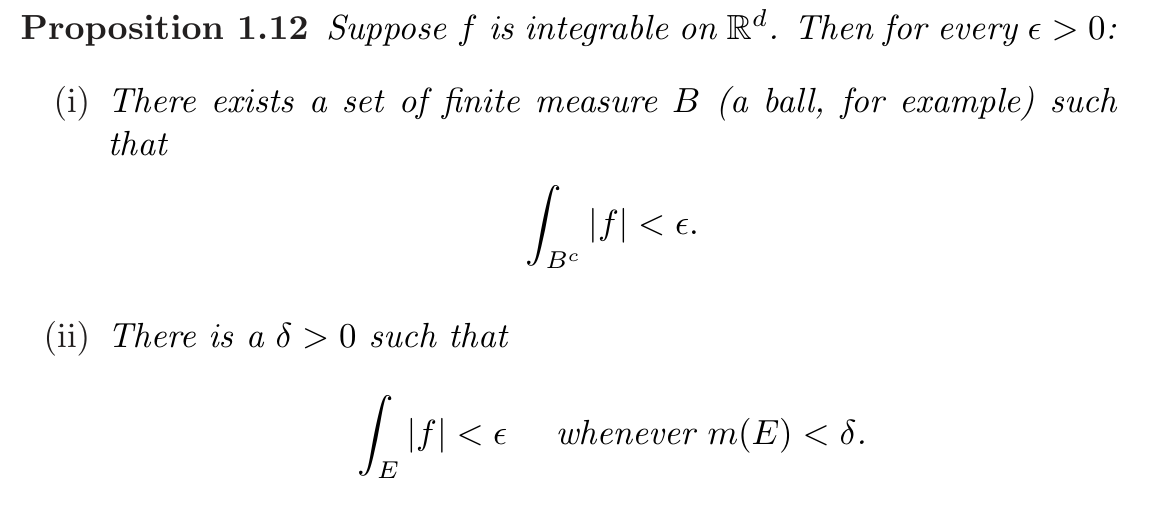
\includegraphics[width=\textwidth]{1-hw13-2025060311.png}
% \caption{}
\label{}
\end{figure}
\begin{figure}[H]
\centering
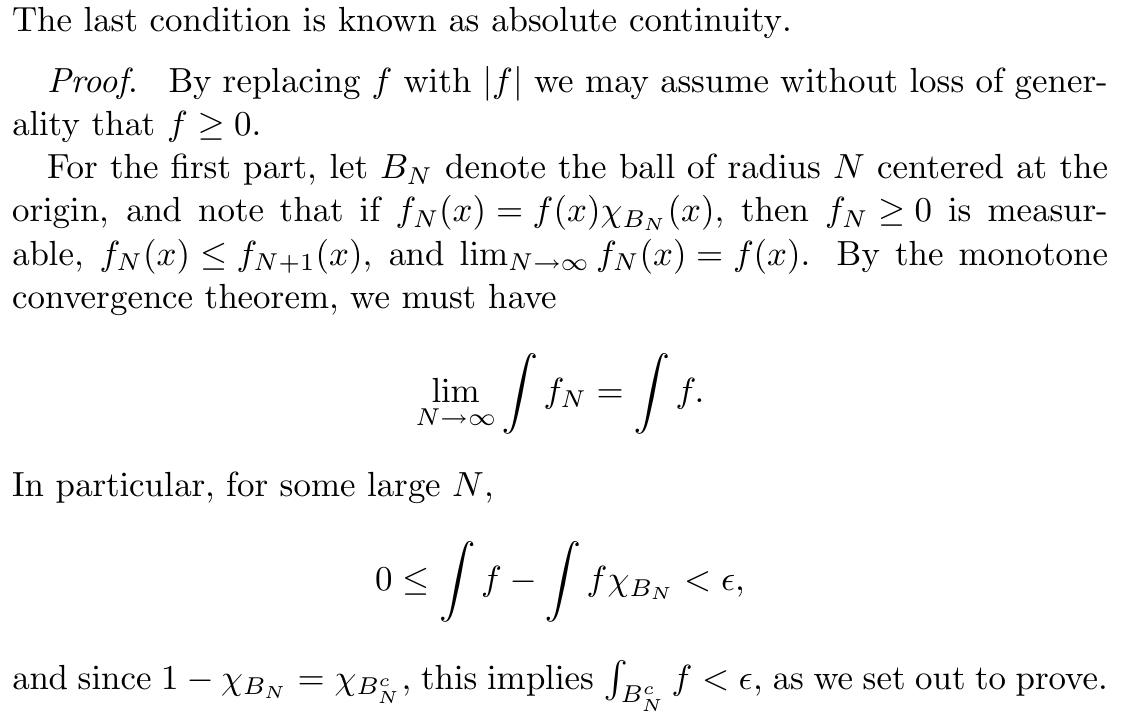
\includegraphics[width=\textwidth]{2-hw13-2025060311.png}
% \caption{}
\label{}
\end{figure}
\begin{figure}[H]
\centering
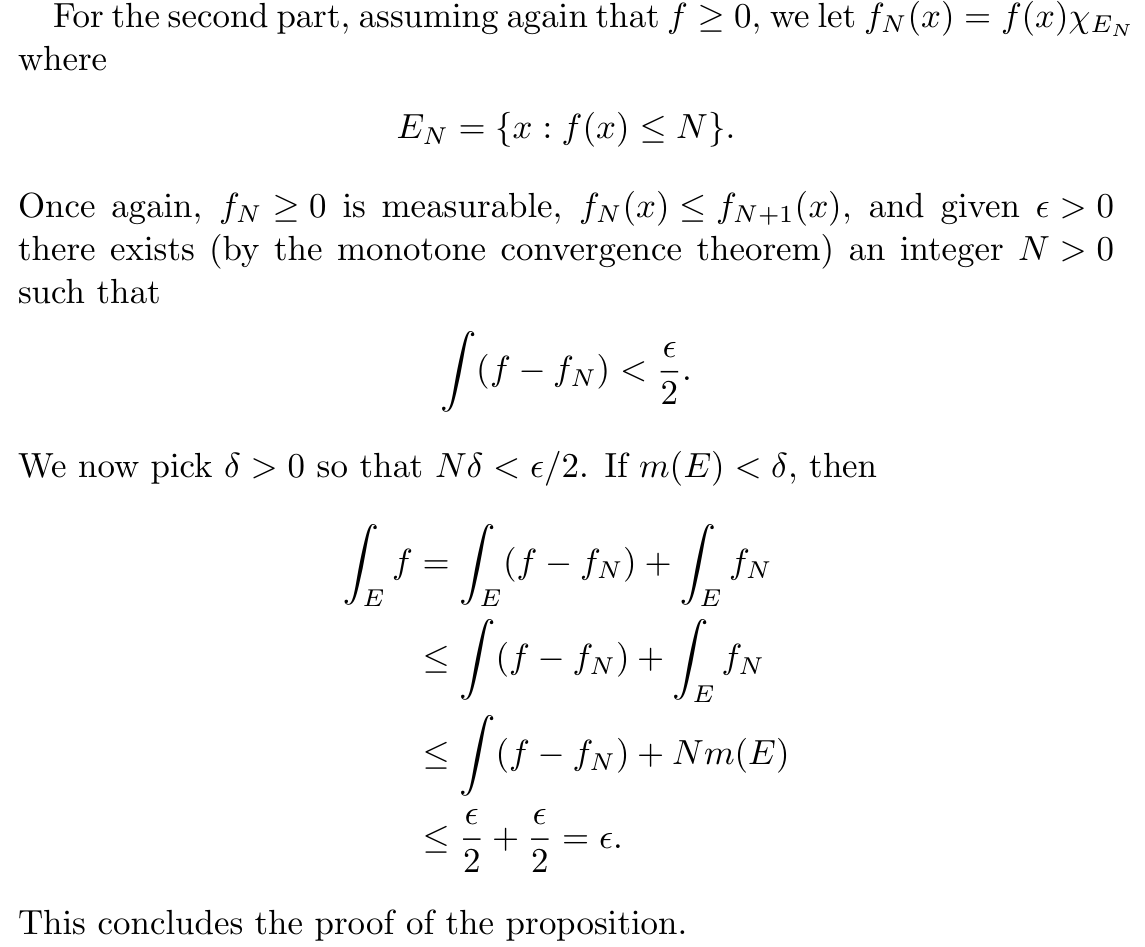
\includegraphics[width=\textwidth]{4-hw13-2025060311.png}
% \caption{}
\label{}
\end{figure}
\end{remark}
\begin{exercise}
\begin{figure}[H]
\centering
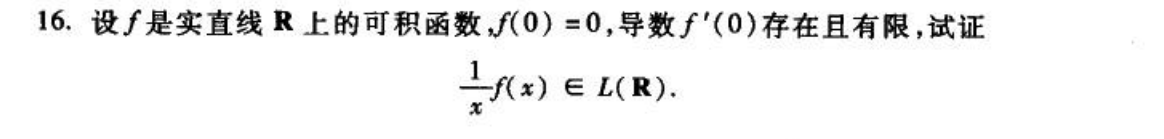
\includegraphics[width=\textwidth]{5-hw13-2025060311.png}
% \caption{}
\label{}
\end{figure}
\end{exercise}
As $x\to0$,
\[
f(x)=\underbrace{ f(0) }_{ =0 }+f'(0)x+o(x)
\]
Then there exists $\delta>0$, s.t. for any $x\in[-\delta,\delta]$,
\[
\lvert f(x)-f'(0)x \rvert \leq \lvert x \rvert
\]
Then
\[
\int_{[-\delta,\delta]}^{} \left\lvert  \frac{1}{x}f(x)  \right\rvert  \, \mathrm{d}x \leq \int_{[-\delta,\delta]}^{} \left\lvert  \frac{1}{x}(\lvert f'(0) \rvert \lvert x \rvert +\lvert x \rvert )  \right\rvert  \, \mathrm{d}x =2\delta(\lvert f'(0) \rvert +1)
\]
\[
\int_{(-\infty,-\delta)\cup(\delta,\infty)}^{} \left\lvert  \frac{1}{x}f(x)  \right\rvert  \, \mathrm{d}x \leq \frac{1}{\delta}\lVert f \rVert _{L^{1}}<\infty
\]
Then
\[
\int_{\mathbb{R}}^{} \left\lvert  \frac{1}{x}f(x)  \right\rvert  \, \mathrm{d}x <\infty
\]
$\frac{1}{x}f(x)$ is absolute integrable over $\mathbb{R}$, thus $\frac{1}{x}f (x)\in L^{1}(\mathbb{R})$.

\begin{exercise}
\begin{figure}[H]
\centering
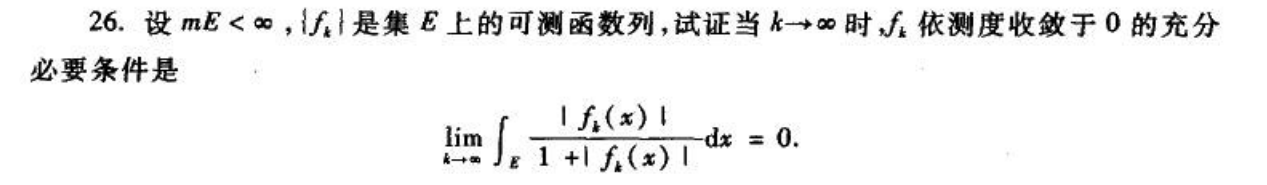
\includegraphics[width=\textwidth]{6-hw13-2025060311.png}
% \caption{}
\label{}
\end{figure}
\end{exercise}
For any $\epsilon>0$, we have $m(E(\lvert f_k \rvert>\epsilon))\to0$ as $k\to \infty$. Then
\[
\begin{aligned}
\left\lvert  \int_{E}^{} \frac{\lvert f_k(x) \rvert }{1+\lvert f_k(x) \rvert } \, \mathrm{d}x   \right\rvert  & \leq \int_{E(\lvert f_k \rvert >\epsilon)}^{} \underbrace{ \frac{\lvert f_k(x) \rvert }{1+\lvert f_k(x) \rvert } }_{ \leq 1 }  \, \mathrm{d}x  +\int_{E(\lvert f_k \rvert \leq \epsilon)}^{}\underbrace{  \frac{\lvert f_k(x) \rvert }{1+\lvert f_k(x) \rvert } }_{ \leq \lvert f_k(x) \rvert \leq \epsilon } \, \mathrm{d}x  \\
 & \leq m(E(\lvert f_k \rvert >\epsilon)) +\epsilon \cdot m(E) \\
 & \to \epsilon \cdot m(E) \qquad \text{as }k\to \infty
\end{aligned}
\]
Since $\epsilon$ is arbitrary,
\[
\lim_{ k \to \infty } \int_{E}^{} \frac{\lvert f_k(x) \rvert }{1+\lvert f_k(x) \rvert } \, \mathrm{d}x =0
\]
\begin{exercise}
\begin{figure}[H]
\centering
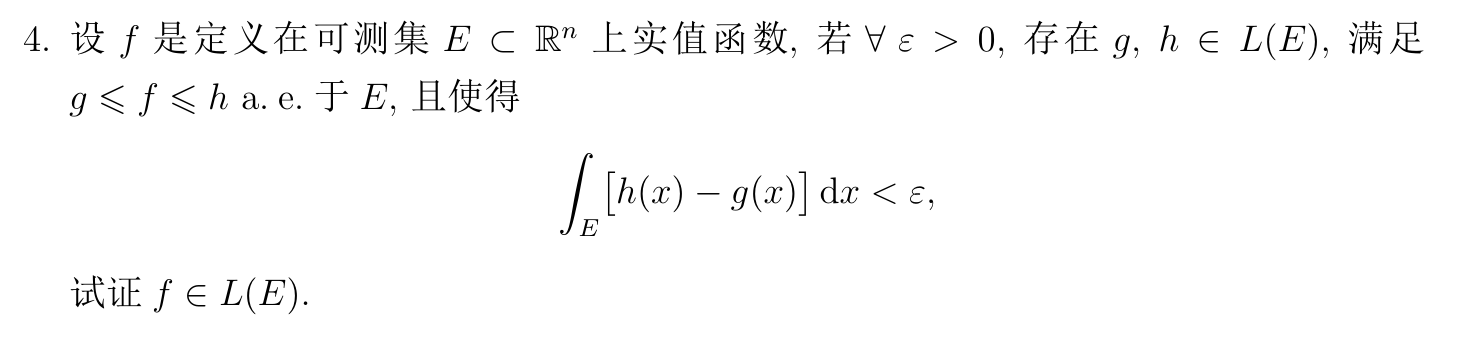
\includegraphics[width=\textwidth]{7-hw13-2025060311.png}
% \caption{}
\label{}
\end{figure}
\end{exercise}
\[
\begin{aligned}
\lVert f \rVert _{L^{1}(E)} & \leq \lVert g \rVert _{L^{1}(E)} +\lVert f-g \rVert _{L^{1}(E)} \\
 & \leq \lVert g \rVert _{L^{1}(E)}+\lVert h-g \rVert _{L^{1}(E)} \\
 & \leq 2\lVert g \rVert _{L^{1}(E)}+\lVert h \rVert _{L^{1}(E)} \\
 & <\infty
\end{aligned} 
\]
Thus $f\in L(E)$.

\begin{exercise}
\begin{figure}[H]
\centering
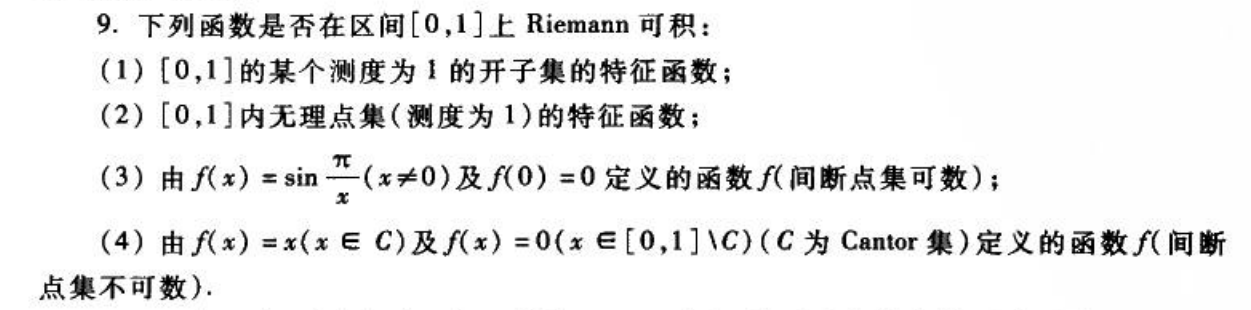
\includegraphics[width=\textwidth]{hw13-2025060312.png}
% \caption{}
\label{}
\end{figure}
\end{exercise}
\begin{figure}[H]
\centering
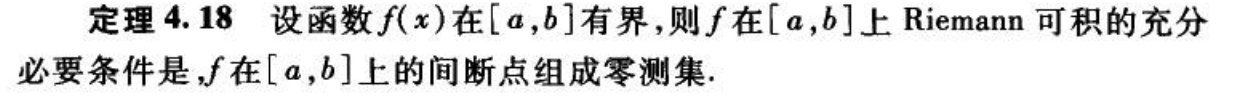
\includegraphics[width=\textwidth]{1-hw13-2025060312.png}
% \caption{}
\label{}
\end{figure}
(1) yes. Suppose $f=\chi_{E}$, where $mE=1$, $E$ is open subset of $[0,1]$. Denote $F\coloneqq[0,1]\setminus E$. The boundary
\[
\partial E=\overline{E}\cap  \overline{([0,1]\setminus E)}=\overline{E}\cap \overline{F}=\overline{E}\cap F\subset F
\]
then $m(\partial E)\leq m(F)=0$, $m(\partial E)=0$. $\partial E$ is the set of discontinuities of $f$, thus $f$ is Riemann integrable.

(2) no. The set of discontinuities is $[0,1]$.

(3) yes. The set of discontinuities  is of measure 0.

(4) yes. The set of discontinuities  is $C$, which is of measure 0.

\begin{exercise}
\begin{figure}[H]
\centering
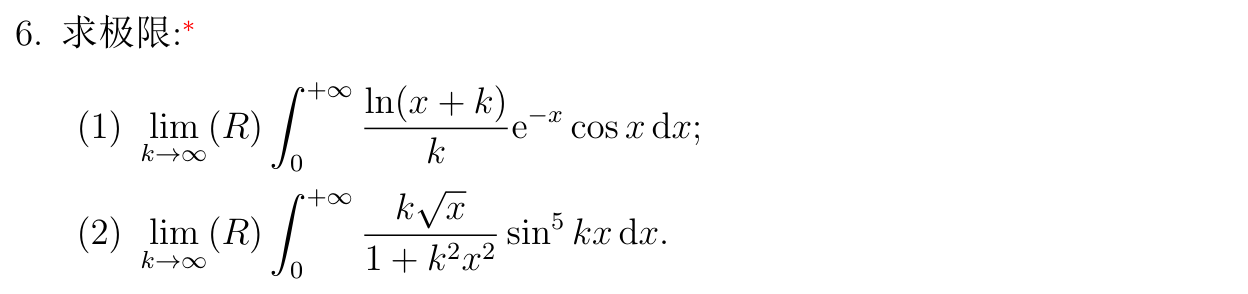
\includegraphics[width=\textwidth]{2-hw13-2025060312.png}
% \caption{}
\label{}
\end{figure}
\end{exercise}
\begin{figure}[H]
\centering
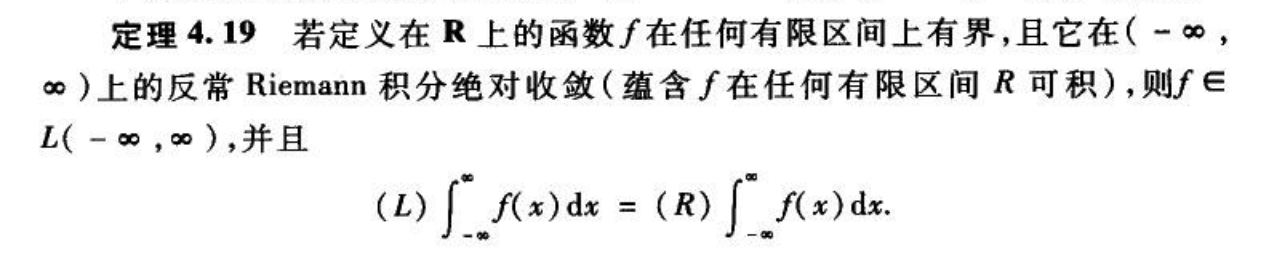
\includegraphics[width=\textwidth]{8-hw13-2025060312.png}
% \caption{}
\label{}
\end{figure}
\begin{figure}[H]
\centering
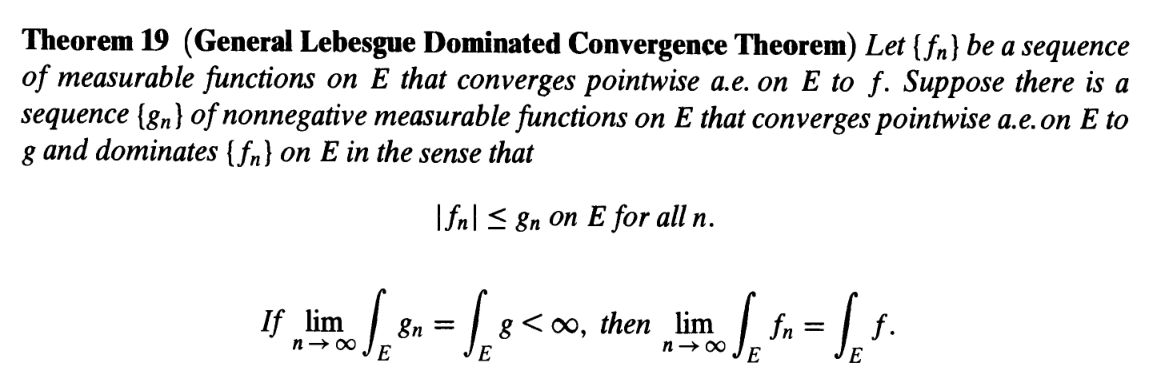
\includegraphics[width=\textwidth]{7-hw13-2025060312.png}
% \caption{}
\label{}
\end{figure}

(1) $f_k(x)=\frac{\ln(x+k)}{k}e^{ -x }\cos x$ is bounded over any finite intevals. Since
\[
\lvert f_k(x) \rvert \leq \frac{x+k}{k}e^{ -x }
\]
and $\int_{0}^{\infty} \frac{x+k}{k}e^{ -x } \, \mathrm{d}x=\frac{1}{k}+1<\infty$, then $f_k$ is absolutelyl integrable over $(0,\infty)$. Thus $f_k\in L(0,\infty)$, and
\[
(L)\int_{0}^{\infty} f_k(x) \, \mathrm{d}x =(R)\int_{0}^{\infty} f_k(x) \, \mathrm{d}x
\]
Then we can apply the General Lebesgue Dominated Convergence Theorem, $g_k(x)\coloneqq\frac{x+k}{k}e^{ -x }$ and $g(x)=e^{ -x }$. We have
\[
\lim_{ k \to \infty } (L)\int_{0}^{\infty} g_k(x) \, \mathrm{d}x =\lim_{ k \to \infty } \left( \frac{1}{k}+1 \right)=1=(L)\int_{0}^{\infty} g(x) \, \mathrm{d}x  <\infty
\]
Then
\[
\lim_{ k \to \infty } (L)\int_{0}^{\infty} f_k(x) \, \mathrm{d}x =(L)\int_{0}^{\infty} \lim_{ k \to \infty } f_k(x) \, \mathrm{d}x =(L)\int_{0}^{\infty} 0 \, \mathrm{d}x =0 
\]
i.e.
\[
\lim_{ k \to \infty } (R)\int_{0}^{\infty} f_k(x) \, \mathrm{d}x =0
\]
(2)
Similar to (1), let $g_k(x)\coloneqq\frac{k\sqrt{ x }}{1+k^2x^2}$, then apply General Lebesgue Dominated Convergence Theorem, we have
\[
\lim_{ k \to \infty } (R)\int_{0}^{\infty} f_k(x) \, \mathrm{d}x =0
\]
\begin{exercise}
\begin{figure}[H]
\centering
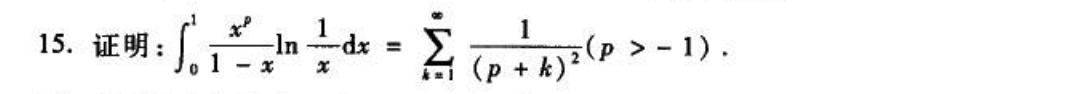
\includegraphics[width=\textwidth]{3-hw13-2025060312.png}
% \caption{}
\label{}
\end{figure}
\end{exercise}
\[
\int_{0}^{1} \frac{x^{p}}{1-x}\ln\frac{1}{x} \, \mathrm{d}x= \int_{0}^{1} \sum_{k=0}^{\infty} \underbrace{ x^{k+p}\ln\frac{1}{x} }_{ \geq 0 } \, \mathrm{d}x \overset{ \text{Levi} }{ = }\sum_{k=0}^{\infty} \int_{0}^{1} x^{k+p}\ln\frac{1}{x} \, \mathrm{d}x =\sum_{k=0}^{\infty } \frac{1}{(1+k+p)^2}=\sum_{k=1}^{\infty} \frac{1}{(k+p)^2}
\]
\begin{exercise}
\begin{figure}[H]
\centering
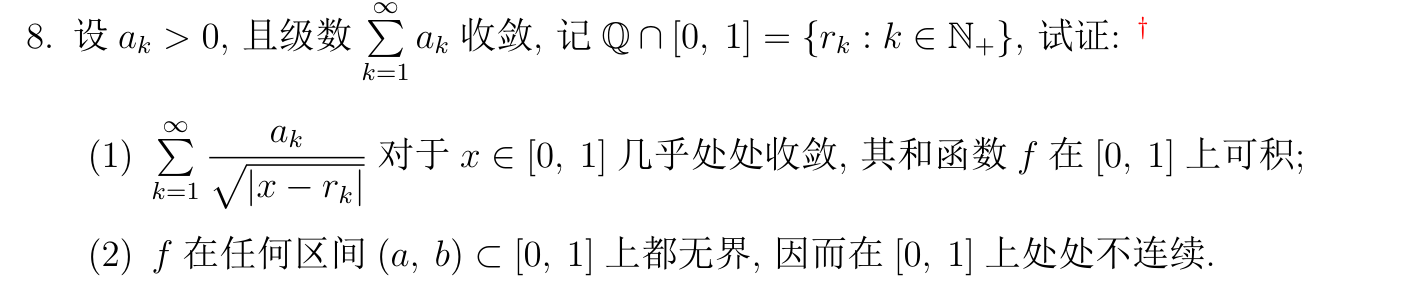
\includegraphics[width=\textwidth]{4-hw13-2025060312.png}
% \caption{}
\label{}
\end{figure}
\end{exercise}
(1)
\[
\begin{aligned}
\int_{0}^{1} \sum_{k=1}^{\infty} \frac{a_k}{\sqrt{ \lvert x-r_k \rvert  }} \, \mathrm{d}x  & \overset{ \text{levi} }{ = }\sum_{k=1}^{\infty}a_k \int_{0}^{1} \frac{1}{\sqrt{ \lvert x-r_k \rvert  }} \, \mathrm{d}x  \\
 & =\sum_{k=1}^{\infty} a_k\left[ \int_{0}^{r_k} \frac{1}{\sqrt{ r_k-x }} \, \mathrm{d}x+\int_{r_k}^{1} \frac{1}{\sqrt{ x-r_k }} \, \mathrm{d}x   \right] \\
 & =\sum_{k=1}^{\infty} a_k\left[ 2 \sqrt{1-r_k}+2 \sqrt{r_k} \right] \\
 & \leq 2\sqrt{ 2 }\sum_{k=1}^{\infty} a_k \\
 & <\infty
\end{aligned}
\]
故 $f (x)=\sum_{k=1}^{\infty}\frac{a_k}{\sqrt{ \lvert x-r_k \rvert }}\in L^{1}[0,1]$,故 $f$ 几乎处处有限,由于 $\frac{a_k}{\sqrt{ \lvert x-r_k \rvert }}\geq0,\forall k$,所以 $\sum_{k=1}^{\infty}\frac{a_k}{\sqrt{ \lvert x-r_k \rvert }}$ 几乎处处收敛.

(2)
任取 $r_n\in(a,b)$,则 $f(x)\geq\frac{a_n}{\sqrt{ \lvert x-r_n \rvert }}$,其中 $a_n>0$,令 $x\to r_n$ 则 $f(x)\geq\frac{a_n}{\sqrt{ \lvert x-r_n \rvert }}\to +\infty$. 故 $f(x)$ 无界. 因此 $f$ 在 $[0,1]$ 处处不连续.

\begin{exercise}
\begin{figure}[H]
\centering
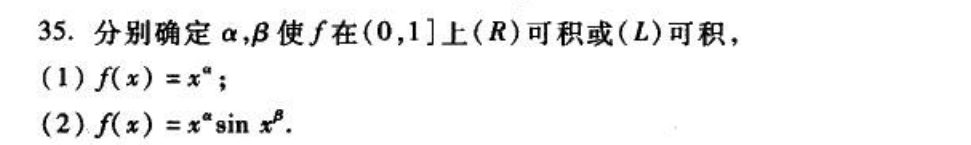
\includegraphics[width=\textwidth]{5-hw13-2025060312.png}
% \caption{}
\label{}
\end{figure}
\end{exercise}
(1) when $\alpha>-1$, $f$ is both Riemann and Lebesgue integrable.

(2) if $\beta\geq0$, then when $\alpha+\beta>-1$, $f$ is both Riemann and Lebesgue integrable.

If $\beta<0$, then $f$ is Riemann integrable iff $\alpha+\beta>-1$, and $f$ is Lebesgue integrable iff $\alpha>-1$.

This is because $(L)\int_{(0,1]}^{} f(x) \, \mathrm{d}x$ exists iff $(R)\int_{(0,1]}^{} \lvert f(x) \rvert \, \mathrm{d}x$ exists, i.e.
\[
\int_{0}^{1} \lvert x^{\alpha}\sin x^{\beta} \rvert  \, \mathrm{d}x
\]
exists. Let $u=x^{\beta}$, then $\int_{0}^{1} \lvert f(x) \rvert \, \mathrm{d}x=\int_{0}^{1} \lvert u \rvert ^{\alpha/\beta }\lvert \sin u \rvert \, \mathrm{d}u^{1/\beta }=\int_{0}^{1} \frac{1}{\beta}u^{\alpha/\beta+1/\beta-1}\lvert \sin u \rvert \, \mathrm{d}u$. It exists iff $\alpha/\beta+1/\beta-1>-1$ i.e. $\alpha>-1$.

\begin{exercise}
\begin{figure}[H]
\centering
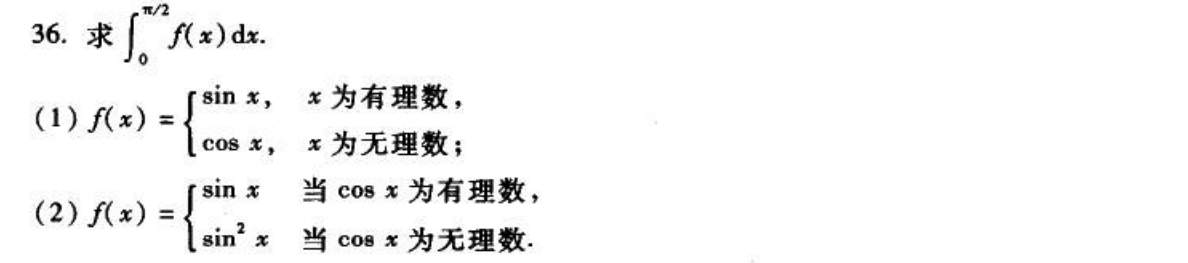
\includegraphics[width=\textwidth]{6-hw13-2025060312.png}
% \caption{}
\label{}
\end{figure}
\end{exercise}
(1)
在零测集上改变函数值不改变积分值
\[
\int_{0}^{\pi/2 } f(x) \, \mathrm{d}x =\int_{0}^{\pi/2 } \cos x \, \mathrm{d}x =1
\]
(2)
由于 $\cos x$ 在 $\left[ 0,\frac{\pi}{2} \right]$ 是双射,所以
\[
\#\left\{  x\in\left[ 0,\frac{\pi}{2} \right]:\cos x\in \mathbb{Q}  \right\}=\#(\mathbb{Q}\cap[0,1])
\]
故 $\left\{  x\in\left[ 0,\frac{\pi}{2} \right]:\cos x\in \mathbb{Q}  \right\}$ 可数,故
\[
\int_{0}^{\pi/2 } f(x) \, \mathrm{d}x=\int_{0}^{\pi/2 } \sin ^2x \, \mathrm{d}x =\frac{\pi}{4}
\]